\documentclass[a4paper,11pt]{article}

\usepackage{fullpage}
\usepackage{color}
\usepackage{hyperref}
\usepackage{amsmath}
\usepackage{amssymb}
\usepackage{tikz}
\usepackage{tabularx}
\usepackage{booktabs}
\usepackage{amsmath}
\usepackage{multirow}
\usepackage{layouts}
\usepackage{array}
\usepackage{pgf}
\usepackage{tikz}
\usepackage{epstopdf}
\usepackage{amssymb}
\usepackage{graphics}
\usepackage{fancyhdr}
\usepackage{eucal}
\usepackage{ifthen}
\usepackage{ifpdf}
\usepackage{lmodern}
\usepackage{amsthm}
\usepackage{catoptions} % For \Autoref


\usetikzlibrary{positioning}

\hypersetup{
  colorlinks,%
    citecolor=black,%
    filecolor=black,%
    linkcolor=black,%
    urlcolor=mygreylink     % can put red here to visualize the links
}

\definecolor{hlcolor}{rgb}{1, 0, 0}
\definecolor{mygrey}{gray}{.85}
\definecolor{mygreylink}{gray}{.30}
\textheight=8.6in
\raggedbottom
\addtolength{\oddsidemargin}{-0.375in}
\addtolength{\evensidemargin}{0.375in}
\addtolength{\textwidth}{0.5in}
\addtolength{\topmargin}{-.375in}
\addtolength{\textheight}{0.75in}


\newcommand{\resheading}[1]{{\large \colorbox{mygrey}{\begin{minipage}{\textwidth}{\textbf{#1 \vphantom{p\^{E}}}}\end{minipage}}}}

\newcommand{\mywebheader}{
  \begin{tabular}{@{}p{5in}p{4in}}
  {\resheading{Assignment 2: Single Agent Learning}} & {\Large 5 October, 2012}\\\vspace{0.2cm}
  \end{tabular}}

\begin{document}


\begin{center}
{\LARGE \textbf{Autonomous Agents}}\\ [1em]
\end{center}
\mywebheader

\begin{center}
{\Large By:} \\ \vspace{0.1cm}
{\Large Paris Mavromoustakos} \\  \vspace{0.1cm}
{\Large Georgios Methenitis} \\ \vspace{0.1cm}
{\Large Marios Tzakris}
\end{center}

\section*{Introduction}
there must be an introduction



\section*{Exercise 1}

First, we loaded the given data files \texttt{banana.mat}, and, \texttt{spiral.mat}, each one of them contains two-dimensional data points, represent two different classes. The training set, which we used in order to train our classifier consists of 75\% of data points from class A, appended to 75\% of data points from class B, while the test set contains the remaining 25\% of both classes A and B. Figure~\ref{fig1}, shows the 2-D representation of the two classes of data-points.

\begin{figure}[h!]
  \centering   
      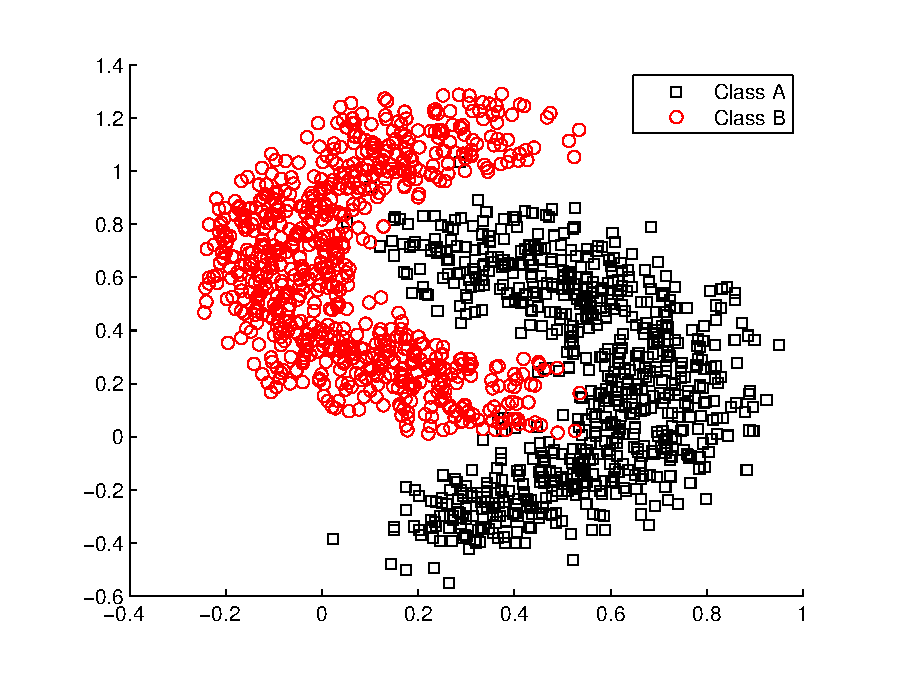
\includegraphics[width=0.49\textwidth]{figures/ABclasses.eps}\		
      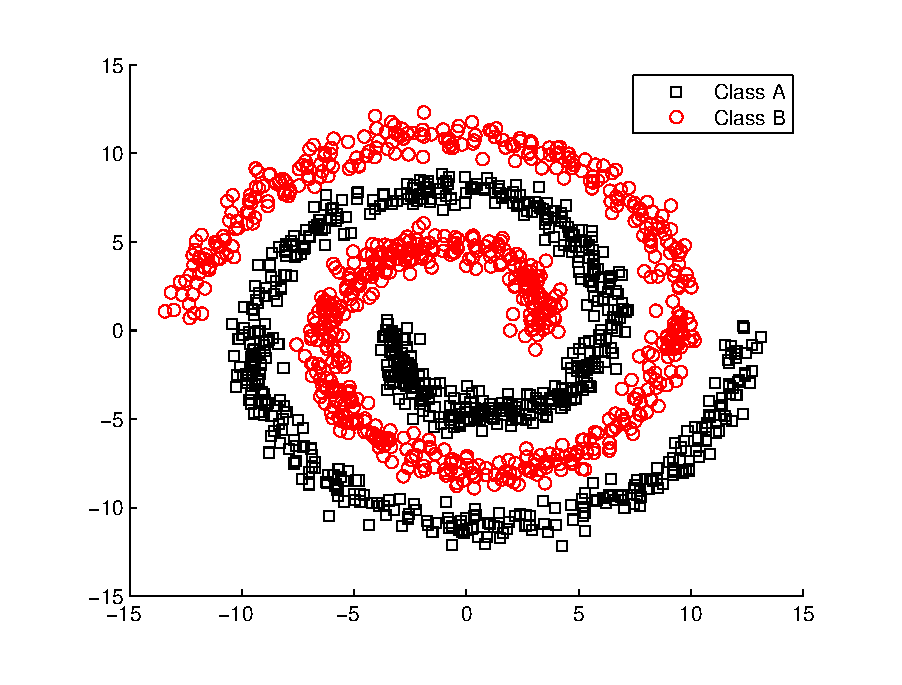
\includegraphics[width=0.49\textwidth]{figures/ABclassesSp.eps}
      
  \caption{Depiction of the 2-D data-points of the two given classes for the \texttt{banana.mat} (left) and \texttt{spiral.mat} (right).}
  \label{fig1}
\end{figure}

Looking into these data-points, we can figure out that the distribution of the data in both cases is following a "banana" and a spiral shape respectively. Therefore, a single 2-D Gaussian distribution could not be able to describe the class conditional probabilities well. For this reason, we do not expect the model to perform accurately. In order to perform the training, we need the prior probabilities, the mean $\mu_k$ of each class and the covariance matrix $\Sigma_k$  for each class $k \in \{A, B\}$. We set the prior probabilities $0.5$ as the number of the data for class A and B is the equal. Next, we can directly extract the mean and and the covariance for each class directly from the training data. The pseudocode for that is given below:\\

\begin{verbatim}
[A, B] = load( data_points )
TrainingSetA = A(1:length(A)*3/4,:)
TrainingSetB = B(1:length(B)*3/4,:)
TrainingSet = [TrainingSetA; TrainingSetB]

prior_probability_A = size(A,1)/(size(A,1)+size(B,1))
prior_probability_B = size(B,1)/(size(A,1)+size(B,1))

for i=1:size(TrainingSetA,1)
   sumAx = sumAx + TrainingSetA(i,1);
   sumAy = sumAy + TrainingSetA(i,2);
   sumBx = sumBx + TrainingSetB(i,1);
   sumBy = sumBy + TrainingSetB(i,2);
end

mean_A = [sumAx sumAy]/size(TrainingSetA,1);
mean_B = [sumBx sumBy]/size(TrainingSetA,1);

covariance_A = cov(TrainingSetA);
covariance_B = cov(TrainingSetB);

pA = mvnpdf(TestSet,mean_A,covariance_A);
pB = mvnpdf(TestSet,mean_B,covariance_B);

PostA = (pA .* prior_probability_A) ./ (pA .* pr_classA + pB .* pr_classB);
PostB = (pB .* prior_probability_B) ./ (pA .* pr_classA + pB .* pr_classB);
\end{verbatim} 
After the classification process we got the following confusion matrices and error rates for the our classifier:
\begin{description}
\item[Banana set]
\begin{align*}
Confusion\ Matrix &= 
\begin{bmatrix}
226 & 24 \\ 
26 & 224
\end{bmatrix},\\
error\ rate &= 0.1
\end{align*}
\item[Spiral set]
\begin{align*}
Confusion\ Matrix &= 
\begin{bmatrix}
174 & 76 \\ 
89 & 161
\end{bmatrix},\\
error\ rate &= 0.33
\end{align*}
\end{description}
As we said before, the way that we tried to perform classification in this type of data, did not perform well, mainly because, the shape of the data, and the fact that, data-points from the one class are located inside the other class, make it impossible for a simple 2-D Gaussian distribution to represent them.



\newpage

\section*{Exercise 2}

\newpage
\section*{Exercise 3}


\newpage
\section*{Conclusion}
\newpage


\end{document}

